\subsection{Безопасность веб"=приложения}

В свете растущих угроз безопасности веб-сервисов особое внимание уделяется надёжным механизмам защиты пользовательских данных. Ключевыми элементами такой защиты являются процессы аутентификации и авторизации, обеспечивающие контроль доступа к ресурсам, а также безопасное хранение паролей с использованием современных методов хэширования. Рассмотрение этих аспектов позволит минимизировать риски несанкционированного доступа и защитить пользователей от компрометации их учётных записей.

\subsubsection{Аутентификация и авторизация (JWT)}

% NOTE: Подводка к JWT
Аутентификация и авторизация --- это фундаментальные компоненты безопасности любой информационной системы, особенно актуальные в области веб"=приложений и сервисов. Они играют решающую роль в защите конфиденциальности и целостности данных, а также в обеспечении контроля доступа к ресурсам и функциям системы.\cite{jwt1}

Аутентификация --- это процесс проверки личности пользователя или устройства, который запрашивает доступ к защищенным ресурсам. Этот процесс включает в себя проверку различных учетных данных, таких как:
\begin{itemize}
	\item{Почта и пароль пользователя: самый распространенный метод аутентификации, который используется для входа в систему.}
	\item{Биометрические данные: распознавание лиц и другие уникальные физиологические характеристики}
	\item{Одноразовые пароли, токены и другие}
\end{itemize}

После успешной аутентификации следует процесс авторизации. Авторизация --- это процесс определения прав пользователя и доступа к ресурсам системы. Этот этап включает в себя:
\begin{itemize}
	\item{Определение доступа: указывает, к каким ресурсам и операциям имеет доступ аутентифицированный пользователь.}
	\item{Управления правами: настраивает уровни доступа, например, разрешение на чтение, запись, редактирование или удаление данных.}
\end{itemize}

Одним из наиболее популярных методов аутентификации является JWT (JSON Web Token).

\textbf{JWT (JSON Web Token)} --- открытый стандарт (RFC 7519) для представления данных в JSON формате между клиентом и сервером.

% NOTE: Структура JWT:

\textbf{Структура JWT:} JWT состоит из трех частей: заголовка, полезной нагрузки и подписи.
\begin{itemize}
	\item{\textbf{Заголовок (header):} часть JWT"=токена, содержащая информацию о типе токена и используемом алгоритме подписи.}
	\item{\textbf{Полезная нагрузка (payload):} часть JWT"=токена, содержащая информацию о пользователе или устройстве, а также дополнительные данные, необходимые для доступа к защищенным ресурсам, например роль}
	\item{\textbf{Подпись (signature):} часть JWT"=токена, гарантирующая целостность токена и подтверждающая его авторство его подлиность.}
\end{itemize}

Схема \ref{fig:JWT} иллюстрирует пример структуры JWT"=токена:

\newpage
\begin{figure}[!h]
    \centering
    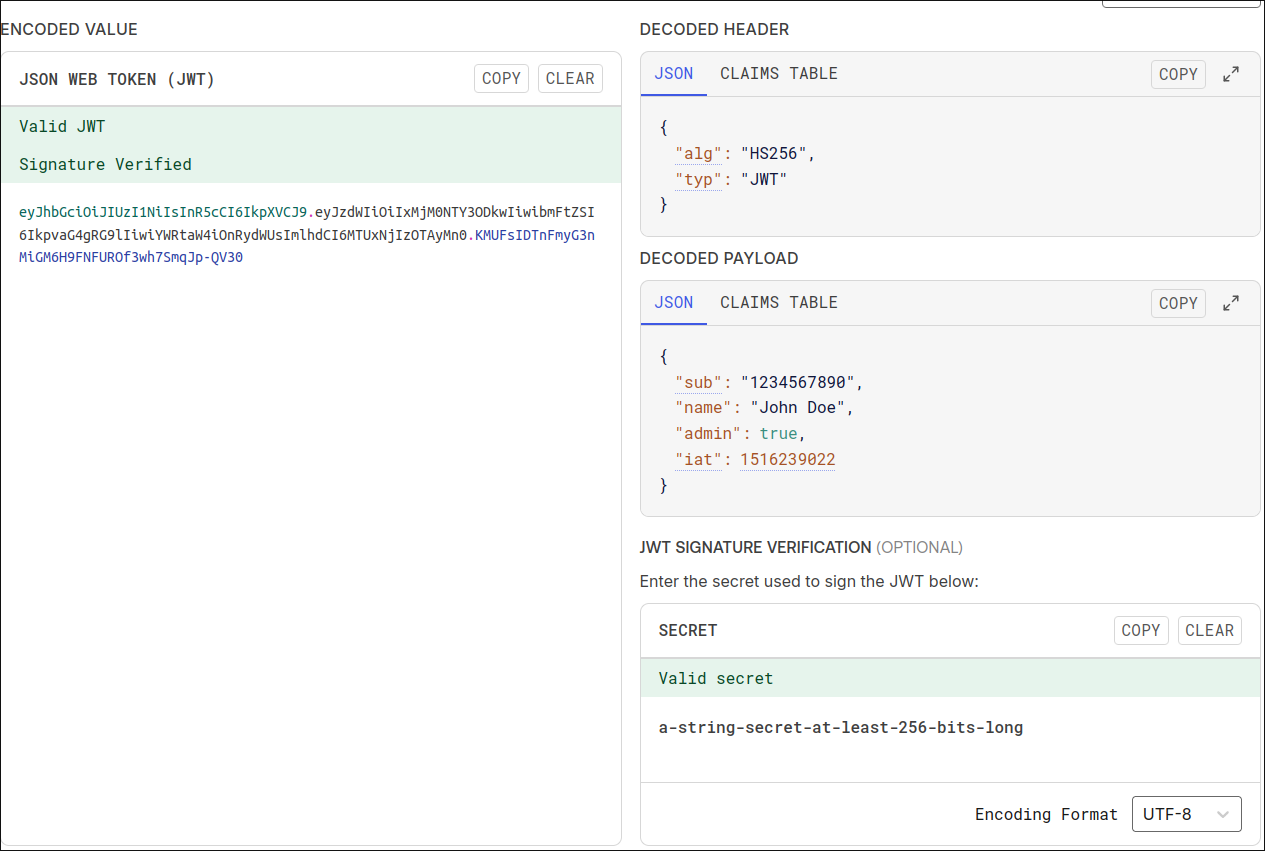
\includegraphics[width = 0.75\textwidth]{imgs/theoryJWT.png}
    \caption{Схема структуры JWT"=токена}
    \label{fig:JWT}
\end{figure}

% NOTE: Принцип использования JWT
Основной принцип использования JWT"=токенов заключается в том, что клиент получает токен после прохождения процесса аутентификации и передает его вместе с каждым запросом к защищенному ресурсу. Сервер в свою очередь, проверяет подлинность токена и разрешает доступ к ресурсу, если токен действителен. Таким образом, JWT"=токены позволяют реализовать механизм авторизации без необходимости хранения состояния на сервере. \cite{jwt2}

% NOTE: Стандарт RFC 7519
Стандарт RFC 7519 определяет несколько типов алгоритмов подписи, которые могут использоваться при создании JWT"=токенов. Некоторые из наиболее распространенных алгоритмов включают HMAC с использованием SHA"=256, RSA и ECDSA. Выбор алгоритма подписи зависит от требований безопасности и возможностей конкретной реализации.

Также стандарт определяет некоторые зарезервированные поля, которые могут использоваться в полезной нагрузке JWT"=токена. Некоторые из этих полей включают идентификатор пользователя (sub), дату истечения срока действия токена (exp), идентификатор клиента (aud).

\subsubsection{Хеширование паролей}

Безопасное хранение паролей пользователей является фундаментальной задачей при разработке систем аутентификации. Существует два способа хранения паролей в базеданных: в чистом виде и в виде зашифрованных значений. 

Хранение в чистом виде --- самый простой способ, при котором пароль хранится точно так, как его ввел пользователь. Это не безопасно, так как в случае утечки данных, злоумышленник может сразу использовать этот пароль.

Более распространённым и безопасным методом является хранение хэшированных паролей. Хэш"=функция --- это функция, которая принимает произвольное количество входных данных и выдает выходные данные фиксированного размера. При этом хэширование является односторонней операцией: восстановить исходный пароль из хэша практически невозможно.

Использование хэш"=функций позволяет хранить не сами пароли, а их хэш"=суммы. В случае компрометации базы данных злоумышленник не сможет напрямую использовать хэши для доступа к аккаунтам. Для повышения безопасности к паролям добавляют случайные данные, называемые солью (salt), что предотвращает атаки с использованием радужных таблиц. Радужная таблица --- это предварительно вычисленный набор хэш"=значений. Эти таблицы позволяют злоумышленникам получать доступ к защищенным системам без подбора пароля.

 Хэш"=функция бывают обратимыми и необратимыми, однако для защиты паролей используют исключительно необратимые функции.

\textbf{Ключеве принципы хеширования паролей:}
\begin{itemize}
	\item{\textbf{Необратимость:} Хэш"=функции должны быть спроектированы так, чтобы обратное преобразование хэша в исходный пароль было невозможно}	
	\item{\textbf{Детерминированность:} Один и тот же пароль всегда генерирует идентичный хэш}
	\item{\textbf{ Соль (salt):} Случайные данные, добавляемые к паролю перед хэшированием для предотвращения атак радужными таблицами}
\end{itemize}
